\documentclass[aspectratio=169,11pt]{beamer}

\usetheme{default}
\usecolortheme{default}
\usepackage{amsmath}
\usepackage{booktabs}
\usepackage{tabularx}
\usepackage{array}
\usepackage{graphicx}

\graphicspath{{assets/}}
\setbeamertemplate{navigation symbols}{}
\setbeamertemplate{footline}[frame number]
\setbeamersize{text margin left=8mm,text margin right=8mm}
\newcolumntype{Y}{>{\raggedright\arraybackslash}X}
\newcommand{\best}[1]{\textbf{#1}}

\title{Bounce Rate Reconstruction from Available Vehicle Sensors}
\subtitle{OU Kalman Filtering, Hybrid Learning, and Model-free Baselines}
\date{August 2026 Monthly Meeting}
\author{}

\begin{document}

\begin{frame}
  \titlepage
  \note{[Sources] docs/claude_explanation/experiment.md; local experiment outputs under lab/kalman_reconstruction/outputs.}
\end{frame}

\begin{frame}{The target signal is unavailable at deployment}
  \begin{columns}[T,onlytextwidth]
    \begin{column}{0.48\textwidth}
      \begin{block}{Deployment constraint}
        \texttt{Bounce\_rate\_6D} cannot be used as an input signal.
      \end{block}

      \begin{itemize}
        \item Reconstruct the 100 Hz Bounce-rate waveform
        \item Use only signals already available on the vehicle
        \item Reserve the unavailable signal for training and evaluation labels
        \item Evaluate on completely held-out drivers
      \end{itemize}
    \end{column}
    \begin{column}{0.48\textwidth}
      \small
      \renewcommand{\arraystretch}{1.25}
      \begin{tabularx}{\textwidth}{@{}p{2.0cm}Yr@{}}
        \toprule
        Group & Available signals & Count\\
        \midrule
        IMU & Roll/yaw rate and 3-axis acceleration & 5\\
        Wheel speed & Four wheel-speed channels & 4\\
        Powertrain & Estimated and commanded torque & 4\\
        \midrule
        Total & Raw input channels & \alert{13}\\
        \bottomrule
      \end{tabularx}
    \end{column}
  \end{columns}

  \vspace{0.35cm}
  \centering
  \textbf{How much accuracy is possible without using Bounce rate at inference?}
  \note{[Sources] lab/kalman_reconstruction/run.py; project Config.x_channels and Config.y_channels.}
\end{frame}

\begin{frame}{Driver-held-out evaluation prevents label leakage}
  \begin{columns}[T,onlytextwidth]
    \begin{column}{0.31\textwidth}
      \centering
      {\LARGE\bfseries 2,429}\\
      Training episodes\\[2mm]
      \small Fitting and normalization
    \end{column}
    \begin{column}{0.31\textwidth}
      \centering
      {\LARGE\bfseries 300}\\
      Validation episodes\\[2mm]
      \small Driver: Cho Hyun-seok\\
      Early stopping
    \end{column}
    \begin{column}{0.31\textwidth}
      \centering
      {\LARGE\bfseries 162}\\
      Held-out test episodes\\[2mm]
      \small Five unseen drivers
    \end{column}
  \end{columns}

  \vspace{0.6cm}
  \begin{block}{Common sequence setup}
    100 Hz sampling, 1,000 samples per episode, and 10 s observation windows.
    Short sequences are edge-padded; long sequences are truncated.
  \end{block}

  \begin{itemize}
    \item Only recorded vehicle data were used; no synthetic data were generated.
    \item Test labels were excluded from fitting, normalization, early stopping, and checkpoint selection.
    \item Final metrics are per-episode correlation, RMSE, and temporal lag.
  \end{itemize}
  \note{[Sources] docs/claude_explanation/experiment.md, Section 2; lab/kalman_reconstruction/run.py.}
\end{frame}

\begin{frame}{Four model families separate interpretability from context access}
  \small
  \renewcommand{\arraystretch}{1.35}
  \begin{tabularx}{\textwidth}{@{}>{\bfseries}p{2.7cm}p{3.2cm}YY@{}}
    \toprule
    Family & Input at inference & Sequence model & Future samples\\
    \midrule
    Model-based
      & Vertical acceleration
      & OU KF
      & No\\
    Hybrid
      & KF states and innovation
      & OU KF + LSTM
      & No\\
    \shortstack[l]{Model-free\\online}
      & 13 sensor channels
      & LSTM, GRU, Transformer
      & No\\
    \shortstack[l]{Model-free\\offline}
      & 13 sensor channels
      & Bi-LSTM, Offline Transformer
      & Yes\\
    \bottomrule
  \end{tabularx}

  \vspace{0.5cm}
  \begin{alertblock}{Comparison boundary}
    KF and hybrid models use vertical acceleration only, whereas model-free models use all 13 channels.
    The final table is therefore a deployment comparison, not an equal-input architecture ablation.
  \end{alertblock}
  \note{[Sources] docs/claude_explanation/experiment.md, Sections 1, 2, and 8.}
\end{frame}

\begin{frame}{OU KF adds a mean-reverting disturbance to a 1-DOF oscillator}
  \begin{columns}[T,onlytextwidth]
    \begin{column}{0.51\textwidth}
      \small
      \textbf{State}
      \[
        \mathbf{x}(t)=
        \begin{bmatrix}z(t)&v(t)&d(t)\end{bmatrix}^{\mathsf T}
      \]

      \textbf{Continuous dynamics}
      \[
        \dot z=v,\qquad
        \dot v=-\omega^2z-2\zeta\omega v+d+w_v
      \]
      \[
        \dot d=-\lambda d+w_d
      \]

      \[
      \mathbf F=
      \begin{bmatrix}
        0&1&0\\
        -\omega^2&-2\zeta\omega&1\\
        0&0&-\lambda
      \end{bmatrix}
      \]
    \end{column}
    \begin{column}{0.45\textwidth}
      \small
      \textbf{Ornstein-Uhlenbeck disturbance}
      \[
        \dot d=-\lambda d+w_d,\qquad
        w_d\sim\mathcal N(0,q_f)
      \]

      \renewcommand{\arraystretch}{1.12}
      \begin{tabularx}{\textwidth}{@{}p{1.1cm}Y@{}}
        $z$ & latent vertical displacement\\
        $v$ & latent vertical velocity\\
        $d$ & OU disturbance acceleration\\
        $f$ & natural frequency, $\omega=2\pi f$\\
        $\zeta$ & damping ratio\\
        $q_v,q_f$ & process-noise intensities\\
        $\lambda$ & mean-reversion rate\\
        $r$ & measurement-noise variance\\
      \end{tabularx}
    \end{column}
  \end{columns}
  \note{[Sources] docs/claude_explanation/experiment.md, Sections 3.2-3.3; lab/kalman_reconstruction/kf.py.}
\end{frame}

\begin{frame}{Continuous-time dynamics are discretized before filtering}
  \small
  The OU model is defined in continuous time, while the data arrive at 100 Hz.
  With $\Delta t=1/100=0.01$ s, define the continuous process-noise matrix
  $\mathbf Q_c=\operatorname{diag}(10^{-10},q_v,q_f)$ and form the Van Loan matrix
  \[
    \mathbf M=\begin{bmatrix}
      \mathbf F & \mathbf Q_c\\
      \mathbf 0 & -\mathbf F^{\mathsf T}
    \end{bmatrix}\Delta t.
  \]

  \[
    e^{\mathbf M}=\begin{bmatrix}
      \mathbf E_{11} & \mathbf E_{12}\\
      \mathbf 0 & \mathbf E_{22}
    \end{bmatrix},
    \qquad
    \mathbf A=\mathbf E_{11},
    \qquad
    \mathbf Q=\mathbf E_{12}\mathbf A^{\mathsf T}.
  \]

  \begin{block}{Discrete model used by the KF}
    \[
      \mathbf x_{k+1}=\mathbf A\mathbf x_k+\mathbf w_k,
      \qquad \mathbf w_k\sim\mathcal N(\mathbf 0,\mathbf Q),
      \qquad y_k=\mathbf C\mathbf x_k+v_k.
    \]
  \end{block}

  \centering
  \footnotesize
  This preserves the continuous-time dynamics and process covariance over one sampling interval;
  it is not an Euler approximation. The implementation stores the resulting discrete $\mathbf Q$ directly.
  \note{[Sources] lecture12.pdf, pp. 13 and 17; docs/claude_explanation/experiment.md, Sections 3.3-3.5; lab/kalman_reconstruction/kf.py.}
\end{frame}

\begin{frame}{One acceleration channel updates all three states online}
  \small
  \textbf{Linear-Gaussian model using the lecture notation}
  \[
    \mathbf x_{t+1}=\mathbf A\mathbf x_t+\mathbf G\mathbf w_t,
    \quad \mathbf w_t\sim\mathcal N(\mathbf 0,\mathbf Q),
    \qquad y_t=\mathbf C\mathbf x_t+v_t,
    \quad v_t\sim\mathcal N(0,\mathbf R)
  \]
  \[
    y_t=9.81(\texttt{IMU\_VerAccelVal}_t-1),\qquad
    \mathbf C=\begin{bmatrix}-\omega^2&-2\zeta\omega&1\end{bmatrix},
    \qquad \mathbf R=\begin{bmatrix}r\end{bmatrix}
  \]

  \begin{columns}[T,onlytextwidth]
    \begin{column}{0.48\textwidth}
      \textbf{Prediction}
      \[
        \hat{\mathbf x}_{t+1|t}=\mathbf A\hat{\mathbf x}_{t|t}
      \]
      \[
        \mathbf P_{t+1|t}=\mathbf A\mathbf P_{t|t}\mathbf A^{\mathsf T}
        +\mathbf G\mathbf Q\mathbf G^{\mathsf T}
      \]

      \textbf{Innovation}
      \[
        \nu_{t+1}=y_{t+1}-\mathbf C\hat{\mathbf x}_{t+1|t}
      \]
      \[
        \mathbf S_{t+1}=\mathbf C\mathbf P_{t+1|t}\mathbf C^{\mathsf T}+\mathbf R
      \]
    \end{column}
    \begin{column}{0.48\textwidth}
      \textbf{Correction}
      \[
        \mathbf K_{t+1}=\mathbf P_{t+1|t}\mathbf C^{\mathsf T}\mathbf S_{t+1}^{-1}
      \]
      \[
        \hat{\mathbf x}_{t+1|t+1}=\hat{\mathbf x}_{t+1|t}
        +\mathbf K_{t+1}\nu_{t+1}
      \]
      \footnotesize
      \[
        \begin{aligned}
        \mathbf P_{t+1|t+1}
          &=(\mathbf I-\mathbf K_{t+1}\mathbf C)\mathbf P_{t+1|t}
            (\mathbf I-\mathbf K_{t+1}\mathbf C)^{\mathsf T}\\
          &\quad+\mathbf K_{t+1}\mathbf R\mathbf K_{t+1}^{\mathsf T}
        \end{aligned}
      \]
    \end{column}
  \end{columns}

  \vspace{0.05cm}
  \centering
  \footnotesize
  The implementation obtains $\mathbf A$ and $\mathbf G\mathbf Q\mathbf G^{\mathsf T}$ at $\Delta t=0.01$ s
  by Van Loan discretization and stores the latter as its discrete $\mathbf Q$ matrix.
  Bounce rate is calibrated as $\hat b_t=g\hat v_{t|t}+c$ using training labels only.
  \note{[Sources] lecture12.pdf, pp. 13 and 17-20; docs/claude_explanation/experiment.md, Sections 3.4-3.7; lab/kalman_reconstruction/kf.py. The lecture symbol C corresponds to the code variable H; the code stores the discrete GQG' covariance as Q.}
\end{frame}

\begin{frame}{The KF parameters optimize reconstruction, not physical identification}
  \begin{columns}[T,onlytextwidth]
    \begin{column}{0.48\textwidth}
      \small
      \textbf{Fitting protocol}
      \begin{itemize}
        \item Up to 300 uniformly sampled training episodes
        \item Powell optimization, at most 40 iterations
        \item Objective: normalized RMSE after affine calibration
      \end{itemize}

      \renewcommand{\arraystretch}{1.1}
      \begin{tabular}{@{}lcc@{}}
        \toprule
        Parameter & Search range & Fitted\\
        \midrule
        $f$ & $0.5$--$8.0$ Hz & $4.0043$\\
        $\zeta$ & $0.05$--$5.0$ & $0.2990$\\
        $q_v$ & $e^{-12}$--$e^3$ & $1.11\!\times\!10^{-3}$\\
        $q_f$ & $e^{-12}$--$e^5$ & $148.4132$\\
        $r$ & $e^{-12}$--$e^4$ & $0.3306$\\
        $\lambda$ & $0.05$--$100$ & $13.4850$\\
        \bottomrule
      \end{tabular}
    \end{column}
    \begin{column}{0.48\textwidth}
      \begin{block}{Held-out result}
        \centering
        \renewcommand{\arraystretch}{1.25}
        \begin{tabular}{@{}lr@{}}
          Median correlation & \textbf{0.9234}\\
          Median RMSE & \textbf{0.2557}\\
          Median lag & \textbf{10 ms}\\
        \end{tabular}
      \end{block}

      \vspace{0.25cm}
      \begin{alertblock}{Interpretation limit}
        The expanded range moved $f$ above the former 3 Hz cap.
        These fitted values are effective reconstruction parameters, not identified suspension properties.
      \end{alertblock}

      \small
      The model is useful as an online reconstruction baseline and as a structured feature generator.
    \end{column}
  \end{columns}
  \note{[Sources] docs/claude_explanation/experiment.md, Sections 3.8-3.9; outputs/ou_lstm_metrics.csv.}
\end{frame}

\begin{frame}{A causal LSTM learns only the KF residual}
  \begin{columns}[T,onlytextwidth]
    \begin{column}{0.55\textwidth}
      \centering
      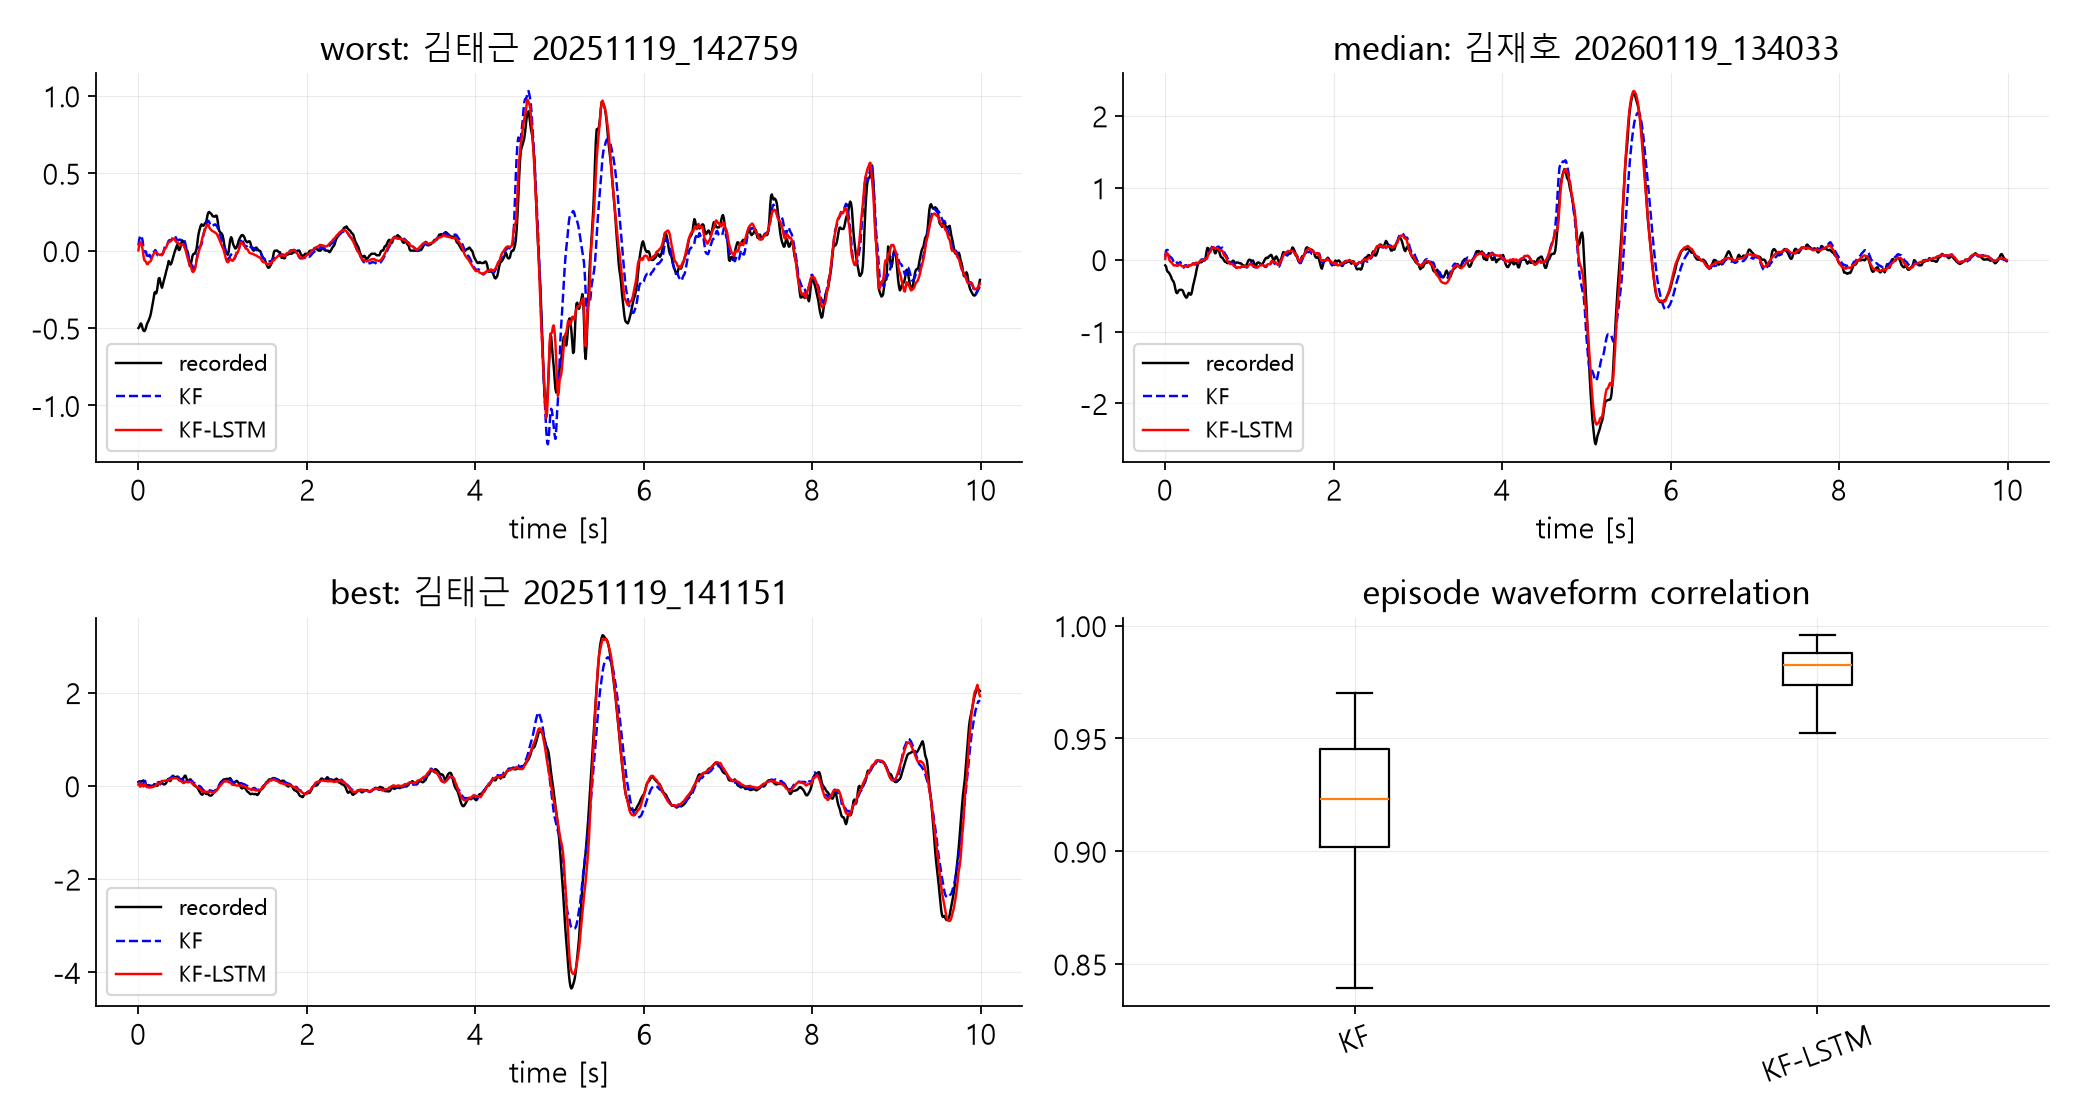
\includegraphics[width=\textwidth,trim=468bp 252bp 0bp 30bp,clip]{ou_lstm_models.png}

      \vspace{0.1cm}
      \small The correction improves both peaks and low-amplitude regions.
    \end{column}
    \begin{column}{0.41\textwidth}
      \small
      \[
        \hat b_k^{\mathrm{hybrid}}=\hat b_k^{\mathrm{KF}}+\Delta\hat b_k^{\mathrm{LSTM}}
      \]
      \[
        \mathbf u_k=[\hat z_k,\hat v_k,\hat d_k,\nu_k]^{\mathsf T}
      \]

      \renewcommand{\arraystretch}{1.08}
      \begin{tabular}{@{}ll@{}}
        LSTM & 2 layers, hidden 64\\
        Head & $64\!\rightarrow\!32\!\rightarrow\!1$, SiLU\\
        Parameters & 52,833\\
        Optimizer & Adam, LR $10^{-3}$\\
        Batch / epochs & 32 / 30 max\\
        Early stopping & Patience 8\\
      \end{tabular}

      \vspace{0.25cm}
      \begin{block}{Median test result}
        Corr. $0.9828$; RMSE $0.1226$; lag $0$ ms.
      \end{block}
      \textbf{RMSE decreases by 52.0\% versus KF alone.}
    \end{column}
  \end{columns}
  \note{[Sources] docs/claude_explanation/experiment.md, Section 4; outputs/ou_lstm_metrics.csv; outputs/ou_lstm_models.png.}
\end{frame}

\begin{frame}{All model-free networks use the same supervised protocol}
  \begin{columns}[T,onlytextwidth]
    \begin{column}{0.49\textwidth}
      \begin{block}{Direct sequence mapping}
        \[
          \hat b_{1:T}=f_{\boldsymbol\phi}(\mathbf s_{1:T}),
          \qquad \mathbf s_t\in\mathbb R^{13}
        \]
      \end{block}

      \small
      \begin{itemize}
        \item Per-channel input z-score from training data
        \item Scalar target mean and standard deviation from training data
        \item Sample-wise MSE on the normalized target
        \item Lowest validation-MSE checkpoint retained
      \end{itemize}
    \end{column}
    \begin{column}{0.47\textwidth}
      \small
      \renewcommand{\arraystretch}{1.18}
      \begin{tabularx}{\textwidth}{@{}p{2.6cm}Y@{}}
        \toprule
        Setting & Value\\
        \midrule
        Optimizer & AdamW\\
        Learning rate & $10^{-3}$\\
        Weight decay & $10^{-4}$\\
        Maximum epochs & 30\\
        LR scheduler & Plateau, factor 0.2, patience 3\\
        Early stopping & Patience 8\\
        Gradient clipping & Norm 5.0\\
        Mixed precision & CUDA only\\
        \bottomrule
      \end{tabularx}
    \end{column}
  \end{columns}

  \vspace{0.35cm}
  \centering
  Online models passed a future-input perturbation test; offline models intentionally use the full episode.
  \note{[Sources] docs/claude_explanation/experiment.md, Section 5; lab/kalman_reconstruction/model_free.py.}
\end{frame}

\begin{frame}{GRU is the strongest model-free online candidate}
  \begin{columns}[T,onlytextwidth]
    \begin{column}{0.55\textwidth}
      \centering
      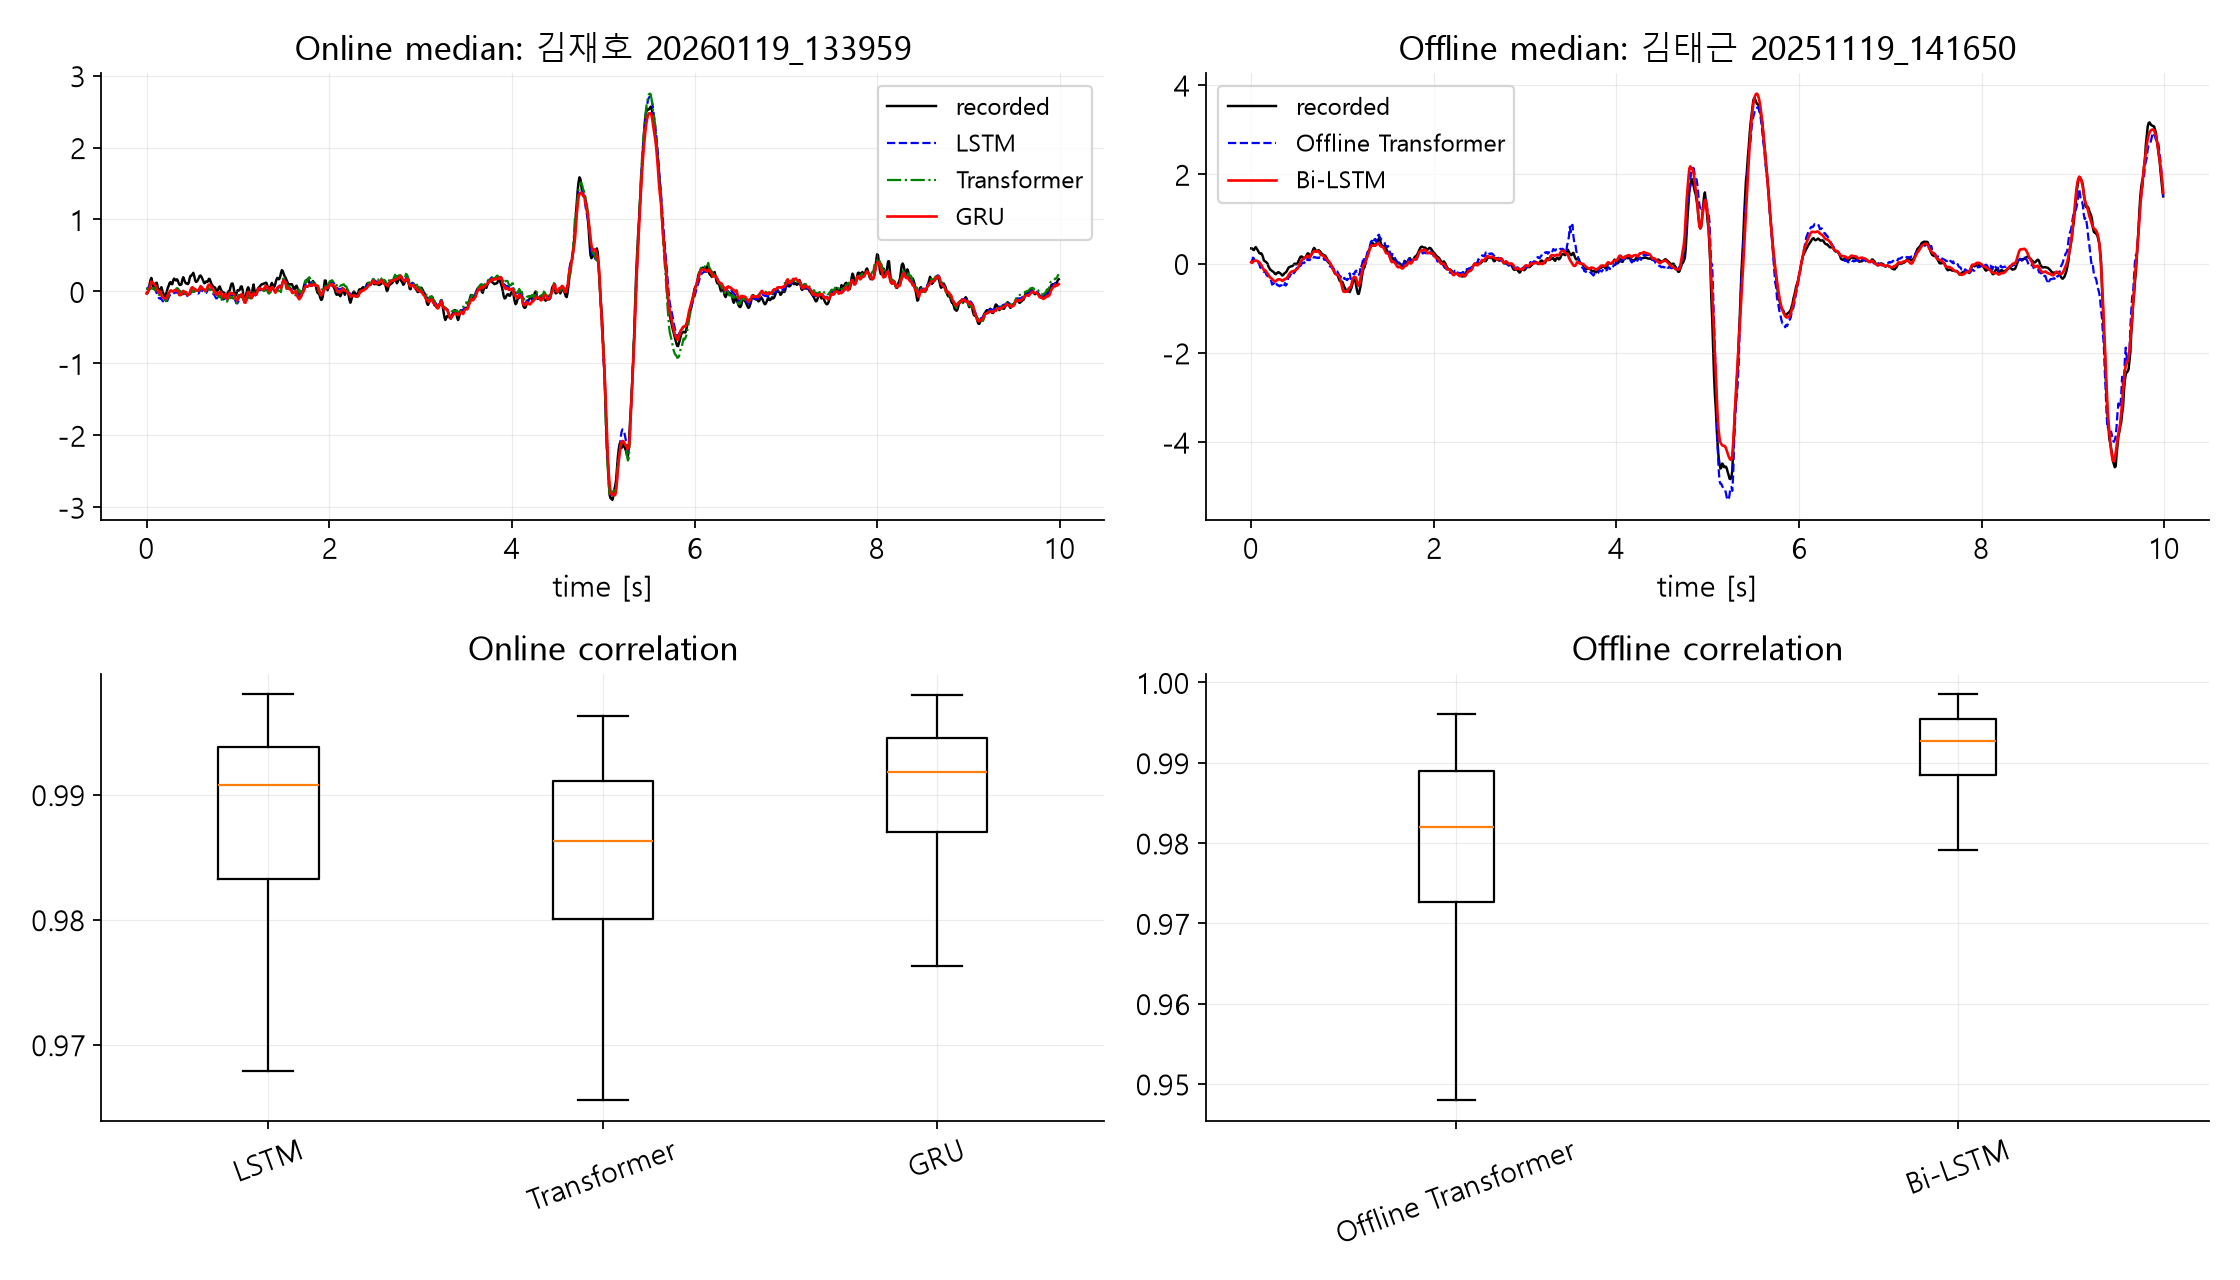
\includegraphics[width=\textwidth,trim=0bp 295bp 504bp 0bp,clip]{model_free_models.png}

      \vspace{0.08cm}
      \small All three models use current and past samples only.
    \end{column}
    \begin{column}{0.42\textwidth}
      \footnotesize
      \setlength{\tabcolsep}{2pt}
      \renewcommand{\arraystretch}{1.1}
      \begin{tabular}{@{}lll@{}}
        \toprule
        Model & Backbone & Params.\\
        \midrule
        LSTM & 2-layer uni., $h=64$ & 53,569\\
        GRU & 2-layer uni., $h=64$ & 40,193\\
        Transformer & 3L, 4H, $d=64$ & 165,505\\
        \bottomrule
      \end{tabular}

      \vspace{0.25cm}
      \begin{tabular}{@{}lrrrr@{}}
        \toprule
        Model & Batch & Epoch & Corr. & RMSE\\
        \midrule
        LSTM & 32 & 28 & 0.9908 & 0.0900\\
        GRU & 32 & 29 & \best{0.9918} & \best{0.0841}\\
        Transformer & 8 & 30 & 0.9863 & 0.1081\\
        \bottomrule
      \end{tabular}

      \vspace{0.25cm}
      \begin{block}{Online choice}
        GRU achieves the lowest error with the fewest parameters.
      \end{block}
    \end{column}
  \end{columns}
  \note{[Sources] docs/claude_explanation/experiment.md, Section 6; outputs/model_free_metrics.csv; outputs/model_free_models.png.}
\end{frame}

\begin{frame}{Bi-LSTM is best overall, but requires the complete episode}
  \begin{columns}[T,onlytextwidth]
    \begin{column}{0.55\textwidth}
      \centering
      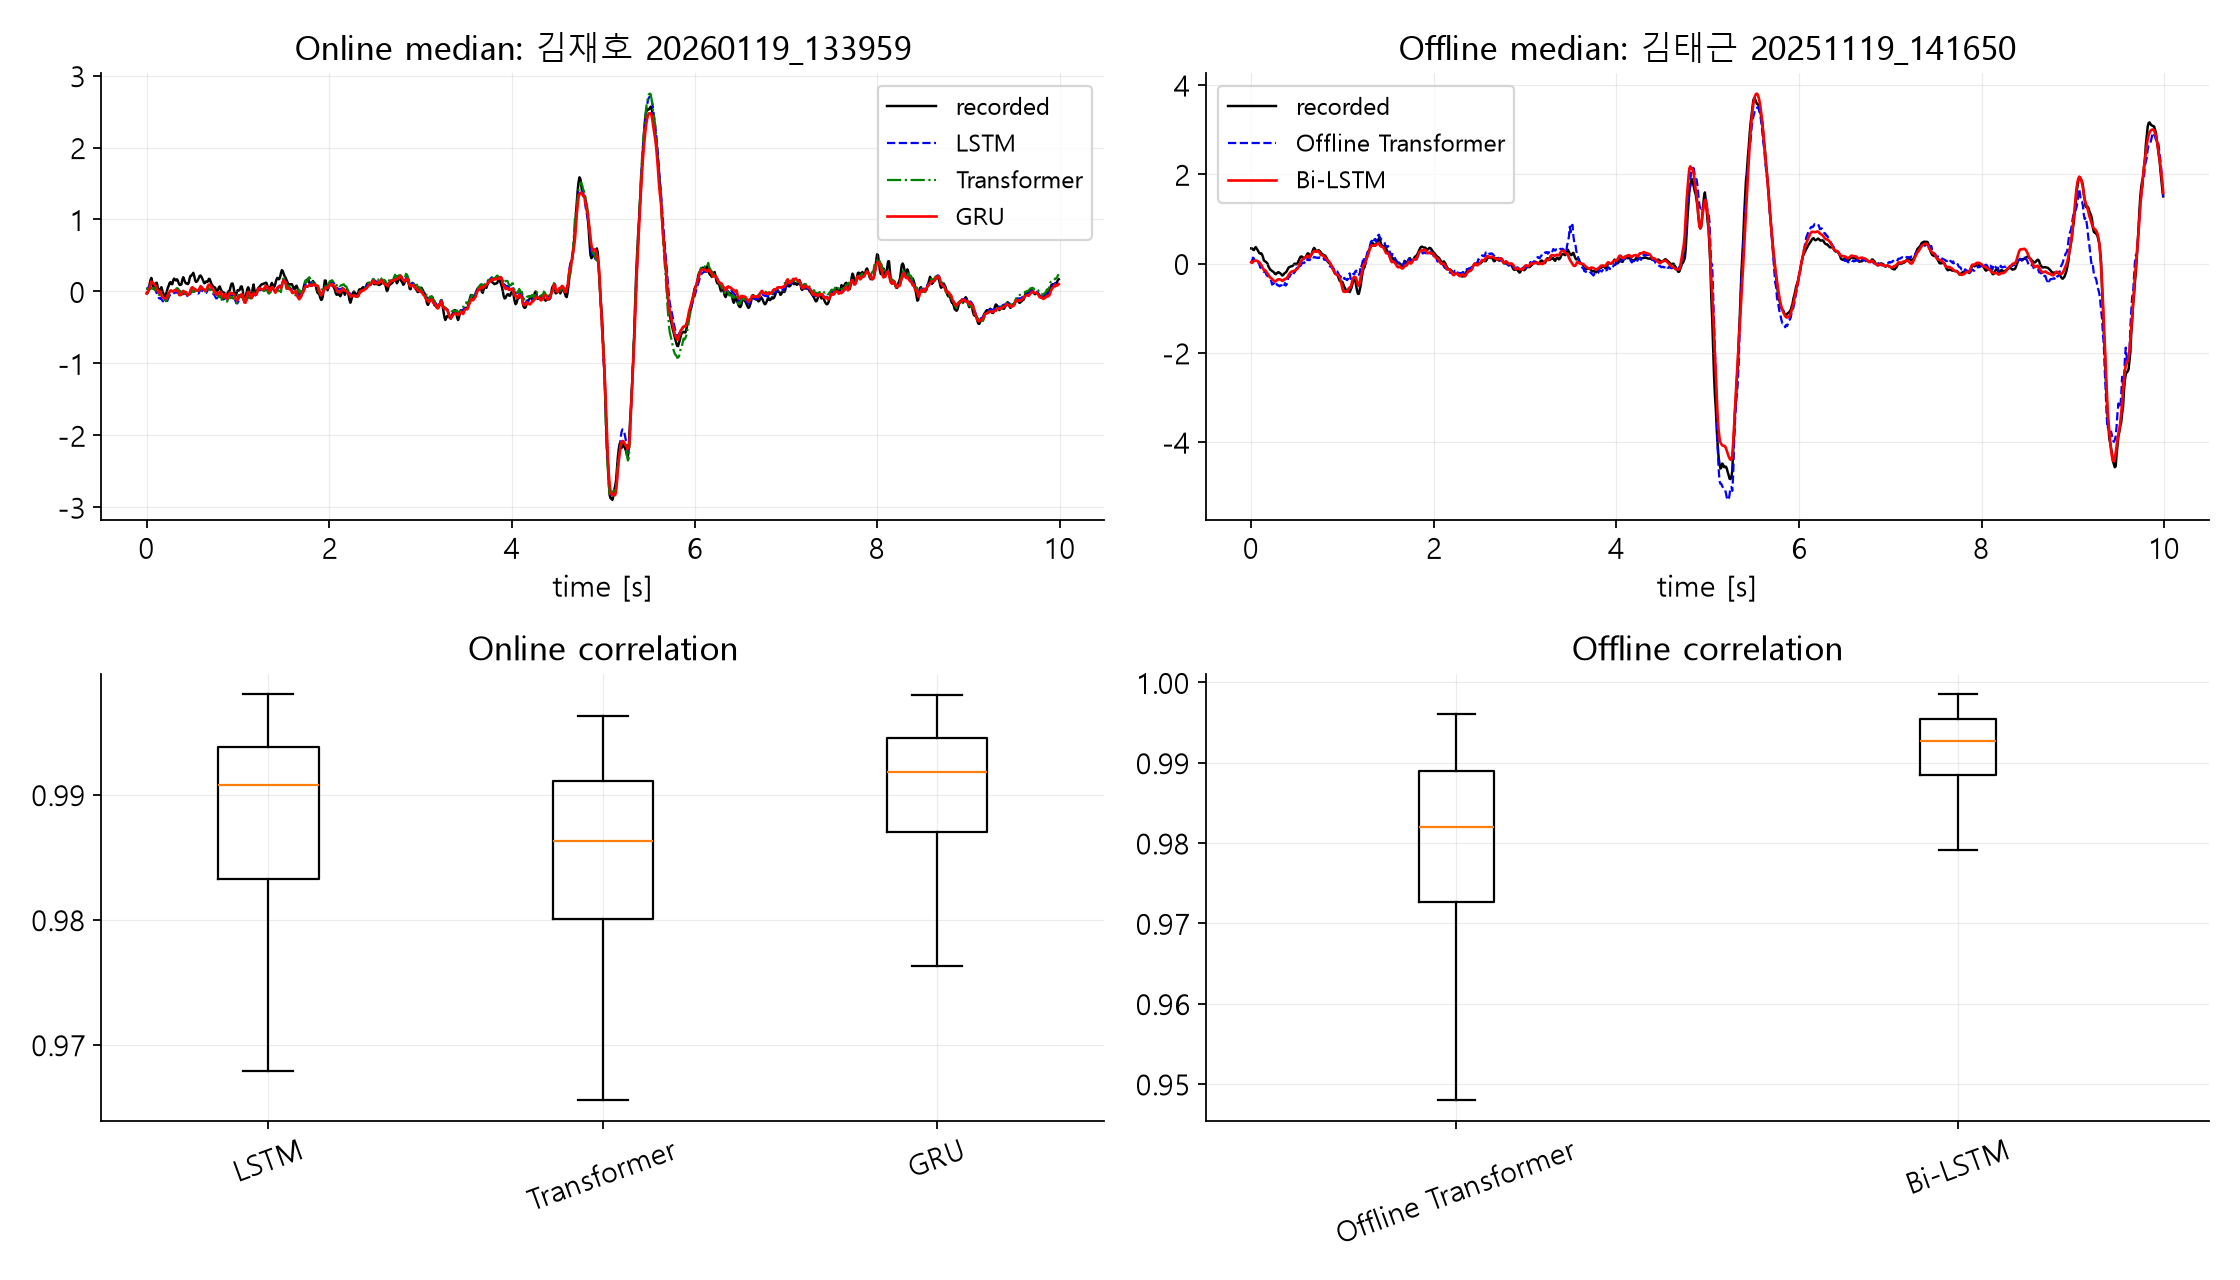
\includegraphics[width=\textwidth,trim=504bp 295bp 0bp 0bp,clip]{model_free_models.png}

      \vspace{0.08cm}
      \small Future context is a capability, not a guarantee of higher accuracy.
    \end{column}
    \begin{column}{0.42\textwidth}
      \footnotesize
      \setlength{\tabcolsep}{2pt}
      \renewcommand{\arraystretch}{1.1}
      \begin{tabular}{@{}lll@{}}
        \toprule
        Model & Backbone & Params.\\
        \midrule
        Bi-LSTM & 2-layer bi., $h=64$ & 139,905\\
        Offline T. & 3L, 4H, $d=64$ & 165,505\\
        \bottomrule
      \end{tabular}

      \vspace{0.25cm}
      \begin{tabular}{@{}lrrrr@{}}
        \toprule
        Model & Batch & Epoch & Corr. & RMSE\\
        \midrule
        Bi-LSTM & 32 & 27 & \best{0.9927} & \best{0.0790}\\
        Offline T. & 8 & 29 & 0.9819 & 0.1203\\
        \bottomrule
      \end{tabular}

      \vspace{0.25cm}
      \begin{block}{Offline choice}
        Bi-LSTM improves median RMSE by 0.0051 over online GRU.
      \end{block}
    \end{column}
  \end{columns}
  \note{[Sources] docs/claude_explanation/experiment.md, Section 7; outputs/model_free_metrics.csv; outputs/model_free_models.png.}
\end{frame}

\begin{frame}{The deployment boundary determines the practical shortlist}
  \small
  \setlength{\tabcolsep}{5pt}
  \renewcommand{\arraystretch}{1.2}
  \begin{tabularx}{\textwidth}{@{}>{\bfseries}p{2.4cm}p{3.3cm}Yrr@{}}
    \toprule
    Role & Model & Main trade-off & Corr. & RMSE\\
    \midrule
    Model-based & KF & One sensor; explicit states & 0.9234 & 0.2557\\
    Hybrid & KF + LSTM & One sensor; learned correction & 0.9828 & 0.1226\\
    Online & \best{GRU} & Best real-time accuracy & 0.9918 & \best{0.0841}\\
    Offline & \best{Bi-LSTM} & Best overall; future context & 0.9927 & \best{0.0790}\\
    \bottomrule
  \end{tabularx}

  \vspace{0.45cm}
  \begin{columns}[T,onlytextwidth]
    \begin{column}{0.48\textwidth}
      \begin{block}{Current evidence}
        Fully model-free recurrent models provide the best accuracy on this held-out split.
      \end{block}
    \end{column}
    \begin{column}{0.48\textwidth}
      \begin{alertblock}{Before final selection}
        Repeat driver splits and seeds, measure inference latency, and run sensor ablation under an equal-input protocol.
      \end{alertblock}
    \end{column}
  \end{columns}
  \note{[Sources] docs/claude_explanation/experiment.md, Section 8; outputs/ou_lstm_metrics.csv; outputs/model_free_metrics.csv.}
\end{frame}

\end{document}
